\chapter{Appendix}

\section{Test Object Variants}


\subsection{IV Position}

\begin{sidewaysfigure}
\begin{multicols}{3}
\begin{center}
\begin{lstlisting}[caption={Position top-head}, language=html, numbers=none]
<!DOCTYPE html>
<html>
    <head>
        <!-- Google Analytics -->
        <script></script>
        <!-- End Google Analytics -->

        <title>
        <meta>
        <link>
        <script>
    </head>

    <body>
        ...
    </body>
</html>
\end{lstlisting}
\end{center}

\columnbreak

\begin{center}
\begin{lstlisting}[caption={Position bottom-head}, language=html, numbers=none]
<!DOCTYPE html>
<html>
    <head>
        <title>
        <meta>
        <link>
        <script>
        
        <!-- Google Analytics -->
        <script></script>
        <!-- End Google Analytics -->
    </head>

    <body>
        ...
    </body>
</html>
\end{lstlisting}
\end{center}

\columnbreak

\begin{center}
\begin{lstlisting}[caption={Position bottom-body}, language=html, numbers=none]
<!DOCTYPE html>
<html>
    <head>
        <title>
        <meta>
        <link>
        <script>
        
    </head>

    <body>
        ...
        <!-- Google Analytics -->
        <script></script>
        <!-- End Google Analytics -->
    </body>
</html>
\end{lstlisting}
\end{center}
\end{multicols}
\end{sidewaysfigure}


\subsection{IV 2 Attribute}

\begin{sidewaysfigure}
\begin{multicols}{3}
\begin{center}
\begin{lstlisting}[caption={Attribute none}, language=html, numbers=none]
<!DOCTYPE html>
<html>
    <head>
        <!-- Google Analytics -->
        <script></script>
        <!-- End Google Analytics -->

        <title>
        <meta>
        <link>
        <script>
    </head>

    <body>
        ...
    </body>
</html>
\end{lstlisting}
\end{center}

\columnbreak

\begin{center}
\begin{lstlisting}[caption={Attribute async}, language=html, numbers=none]
<!DOCTYPE html>
<html>
    <head>
        <!-- Google Analytics -->
        <script async></script>
        <!-- End Google Analytics -->

        <title>
        <meta>
        <link>
        <script>
    </head>

    <body>
        ...
    </body>
</html>
\end{lstlisting}
\end{center}

\columnbreak

\begin{center}
\begin{lstlisting}[caption={Attribute defer}, language=html, numbers=none]
<!DOCTYPE html>
<html>
    <head>
        <!-- Google Analytics -->
        <script defer></script>
        <!-- End Google Analytics -->

        <title>
        <meta>
        <link>
        <script>
    </head>

    <body>
        ...
    </body>
</html>
\end{lstlisting}
\end{center}
\end{multicols}
\end{sidewaysfigure}








\subsection{IV 3 Other Script}

\begin{sidewaysfigure}
\begin{multicols}{2}
\begin{center}
\begin{lstlisting}[caption={Other Script no}, language=html, numbers=none]
<!DOCTYPE html>
<html>
    <head>
        <!-- Google Analytics -->
        <script></script>
        <!-- End Google Analytics -->
        




        <title>
        <meta>
        <link>
        <script>
    </head>

    <body>
        ...
    </body>
</html>
\end{lstlisting}
\end{center}

\columnbreak

\begin{center}
\begin{lstlisting}[caption={Other Script yes}, language=html, numbers=none]
<!DOCTYPE html>
<html>
    <head>
        <!-- Google Analytics -->
        <script></script>
        <!-- End Google Analytics -->
        
        <!-- Other Script-->
        <script></script>
        <!-- End Other Script -->

        <title>
        <meta>
        <link>
        <script>
    </head>

    <body>
        ...
    </body>
</html>
\end{lstlisting}
\end{center}
\end{multicols}
\end{sidewaysfigure}


% ------------------------------------------------------------------------------------------------








% To big to fail / to delete... in the end i will still delete it haha. Too afraid or what ?? Kostet nix es zu behalten. Für alle Fälle...


% \subsection{Single Test Raw page data}

% WPT Metrics from summary file
% \begin{center}
% 	\small
% 	\begin{longtable}{ p{0.4\linewidth} | p{0.6\linewidth} }
% 	Name & Description \\ 
% 	\hline
%         minify\textunderscore total & Total bytes of minifiable text static assets. \\
%         responses\textunderscore 200 & The number of responses with HTTP status code of 200, OK. \\
%         testStartOffset & ... \\
%         bytesOut & The total bytes sent from the browser to other servers. \\
%         gzip\textunderscore savings & Total bytes of compressed responses. \\
%         requestsFull & ... \\
%         start\textunderscore epoch & ... \\
%         connections & The number of connections used. \\
%         base\textunderscore page\textunderscore cdn & The CDN provider for the base page. \\
%         bytesOutDoc & Same as bytesOut but only includes bytes until the Document Complete
% event. Usually when all the page content has loaded (window.onload). \\
%         result & Test result code. \\
%         final\textunderscore base\textunderscore page\textunderscore request\textunderscore id & ... \\
%         basePageSSLTime & ... \\
%         docTime & Same as loadTime. \\
%         domContentLoadedEventEnd & Time in ms since navigation started until document DOMContentLoaded event finished. \\
%         image\textunderscore savings & Total bytes of compressed images. \\
%         requestsDoc & The number of requests until Document Complete event. \\
%         firstMeaningfulPaint & ... \\
%         score\textunderscore cookies & WebPageTest performance review score for not using cookies on static assets. \\
%         firstPaint & RUM First Paint Time, the time in ms when browser first painted something on screen. It's calculated on the client for browsers that implement this method. \\
%         score\textunderscore cdn & WebPageTest performance review score for using CDN for all static assets. \\
%         optimization\textunderscore checked & Whether or not optmizations were checked. \\
%         score\textunderscore minify & WebPageTest performance review score for minifying text static assets. \\
%         gzip\textunderscore total & Total bytes of compressible responses. \\
%         responses\textunderscore 404 & The number of responses with HTTP status code of 404, not found. \\
%         loadTime & The total time taken to load the page (window.onload) in ms. \\
%         URL & The tested page URL. \\
%         score\textunderscore combine & WebPageTest performance review score for bundling JavaScript and/or CSS assets. \\
%         firstContentfulPaint & ... \\
%         image\textunderscore total & Total bytes of images. \\
%         score\textunderscore etags & WebPageTest performance review score for disabling *ETag*s. \\
%         loadEventStart & Time in ms since navigation started until window.onload event was triggered (from W3C Navigation Timing). \\
%         minify\textunderscore savings & Total bytes of minified text static assets. \\
%         score\textunderscore progressive\textunderscore jpeg & WebPageTest performance review score for using progressive JPEG. \\
%         domInteractive & ... \\
%         score\textunderscore gzip & WebPageTest performance review score for using gzip compression for transferring compressable responses. \\
%         score\textunderscore compress & WebPageTest performance review score for compressing images. \\
%         domContentLoadedEventStart & Time in ms since navigation started until document DOMContentLoaded event was triggered (from W3C Navigation Timing). \\
%         final\textunderscore url & ... \\
%         bytesInDoc & Same as bytestIn but only includes bytes until Document Complete event. \\
%         firstImagePaint & ... \\
%         score\textunderscore keep-alive & WebPageTest performance review score for using persistent connections. \\
%         loadEventEnd & Time in ms since navigation started until window.onload event finished. \\
%         cached &  0 for first view or 1 for repeat view. \\
%         score\textunderscore cache & WebPageTest performance review score for leveraging browser caching of static assets. \\
%         responses\textunderscore other & The number of responses with HTTPS status code different from 200 or 404. \\
%         main\textunderscore frame & ... \\
%         fullyLoaded & The time (in ms) the page took to be fully loaded — e.g., 2 seconds of no network activity after Document Complete. This will usually include any activity that is triggered by javascript after the main page loads. \\
%         requests & List of details of all requests on tested page. \\
%         final\textunderscore base\textunderscore page\textunderscore request & ... \\
%         TTFB & Time to first byte, which is the duration in ms from when the user first made the HTTP request to the very first byte of the page being received by the browser. \\
%         bytesIn & The amount of data that browser had to download in order to load the page. It is also commonly referred to as the page size. \\
%         osPlatform & ... \\
%         test\textunderscore run\textunderscore time\textunderscore ms & ... \\
%         tester & The ID of tester that performed the page test. \\
%         browser\textunderscore version & The browser version. \\
%         document\textunderscore origin & ... \\
%         document\textunderscore URL & ... \\
%         date & Time and date (number of seconds since Epoch) when test was complete. \\
%         PerformancePaintTiming.first-paint & ... \\
%         osVersion & ... \\
%         domElements & The total number of DOM elements. \\
%         browserVersion & The browser version. \\
%         fullyLoadedCPUms & CPU busy time in ms until page was fully loaded. \\
%         browser\textunderscore name & The browser name. \\
%         PerformancePaintTiming.first-contentful-paint & ... \\
%         base\textunderscore page\textunderscore cname & ... \\
%         eventName & ... \\
%         os\textunderscore version & ... \\
%         base\textunderscore page\textunderscore dns\textunderscore server & ... \\
%         fullyLoadedCPUpct & Average CPU utilization up until page is fully loaded. \\
%         domComplete & ... \\
%         base\textunderscore page\textunderscore ip\textunderscore ptr & ... \\
%         document\textunderscore hostname & ... \\
%         lastVisualChange & Time in ms until the last visual changed occured. \\
%         visualComplete & Time in ms when page was visually completed. \\
%         render & The first point in time (in ms) that something was displayed to the screen. Before that user was staring at a blank page. This does not necessarily mean the user saw the page content — it could just be something as simple as a background color — but it is the first indication of something happening for the user. \\
%         SpeedIndex & The SpeedIndex score. \\
%         visualComplete85 & Time in ms when page was visually completed 85\%. \\
%         visualComplete90 & Time in ms when page was visually completed 90\%. \\
%         visualComplete95 & Time in ms when page was visually completed 95\%. \\
%         visualComplete99 & Time in ms when page was visually completed 99\%. \\
%         LargestContentfulPaintType & ... \\
%         LargestContentfulPaintNodeType & ... \\
%         chromeUserTiming.navigationStart & ... \\
%         chromeUserTiming.fetchStart & ... \\
%         chromeUserTiming.responseEnd & ... \\
%         chromeUserTiming.domLoading & ... \\
%         chromeUserTiming.markAsMainFrame & ... \\
%         chromeUserTiming.domInteractive & ... \\
%         chromeUserTiming.domContentLoadedEventStart & ... \\
%         chromeUserTiming.domContentLoadedEventEnd & ... \\
%         chromeUserTiming.firstPaint & ... \\
%         chromeUserTiming.firstContentfulPaint & ... \\
%         chromeUserTiming.firstImagePaint & ... \\
%         chromeUserTiming.firstMeaningfulPaint & ... \\
%         chromeUserTiming.firstMeaningfulPaintCandidate & ... \\
%         chromeUserTiming.domComplete & ... \\
%         chromeUserTiming.loadEventStart & ... \\
%         chromeUserTiming.loadEventEnd & ... \\
%         chromeUserTiming.LargestContentfulPaint & ... \\
%         chromeUserTiming.LargestTextPaint & ... \\
%         chromeUserTiming.CumulativeLayoutShift & ... \\
%         run & The run number. \\
%         step & ... \\
%         effectiveBps & Bytes per seconds, i.e.: total of bytes in / total time to load the page. \\
%         effectiveBpsDoc & Same as effectiveBps but until Document Complete event. \\
%         domTime & The total time in ms until a given DOM element (specified via domelement parameter when running a test) was found on the page. \\
%         aft & Above the Fold Time (no longer supported). The time taken to load everything in the viewport above the fold. \\
%         titleTime & Total time in ms until page title was set on browser. \\
%         domLoading & ... \\
%         server\textunderscore rtt & ... \\
%         smallImageCount & ... \\
%         bigImageCount & ... \\
%         maybeCaptcha & ... \\
%         bytes.html & ... \\
%         requests.html & ... \\
%         bytesUncompressed.html & ... \\
%         bytes.js & ... \\
%         requests.js & ... \\
%         bytesUncompressed.js & ... \\
%         bytes.css & ... \\
%         requests.css & ... \\
%         bytesUncompressed.css & ... \\
%         bytes.image & ... \\
%         requests.image & ... \\
%         bytesUncompressed.image & ... \\
%         bytes.flash & ... \\
%         requests.flash & ... \\
%         bytesUncompressed.flash & ... \\
%         bytes.font & ... \\
%         requests.font & ... \\
%         bytesUncompressed.font & ... \\
%         bytes.video & ... \\
%         requests.video & ... \\
%         bytesUncompressed.video & ... \\
%         bytes.other & ... \\
%         requests.other & ... \\
%         bytesUncompressed.other & ... \\
%         id & ... \\
%         chromeUserTiming.InteractiveTime & ... \\
%      \caption{Your caption here} % needs to go inside longtable environment
% 	\label{tab:myfirstlongtable}
% 	\end{longtable}
% \end{center}



\section{Measurement Results}

\subsection{Original Website vs Test Website without GA}

% --- Page Weight FV ---
\begin{figure}
	\centering
	\begin{subfigure}{.5\textwidth}
		\centering
		\includegraphics[width=1\linewidth]{plots/original_vs_test/bytes_fv.pdf}
		%\caption{Bytes First View}
		\label{fig:sub1}
	\end{subfigure}%
	\begin{subfigure}{.5\textwidth}
		\centering
		\includegraphics[width=1\linewidth]{plots/original_vs_test/requests_fv.pdf}
		%\caption{Requests First View}
		\label{fig:sub2}
	\end{subfigure}
	\caption{Page Weight First View, Original vs Test.}
	\label{figure:plt_original_test}
\end{figure}

% --- Page Weight RV ---
\begin{figure}
	\centering
	\begin{subfigure}{.5\textwidth}
		\centering
		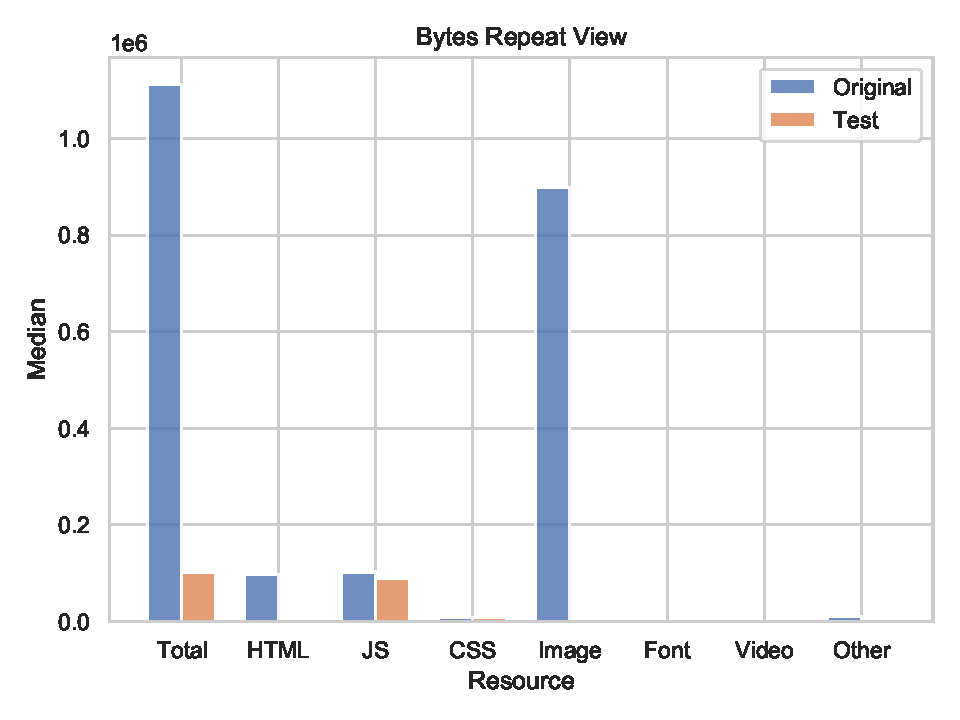
\includegraphics[width=1\linewidth]{plots/original_vs_test/bytes_rv.pdf}
		%\caption{Bytes First View}
		\label{fig:sub1}
	\end{subfigure}%
	\begin{subfigure}{.5\textwidth}
		\centering
		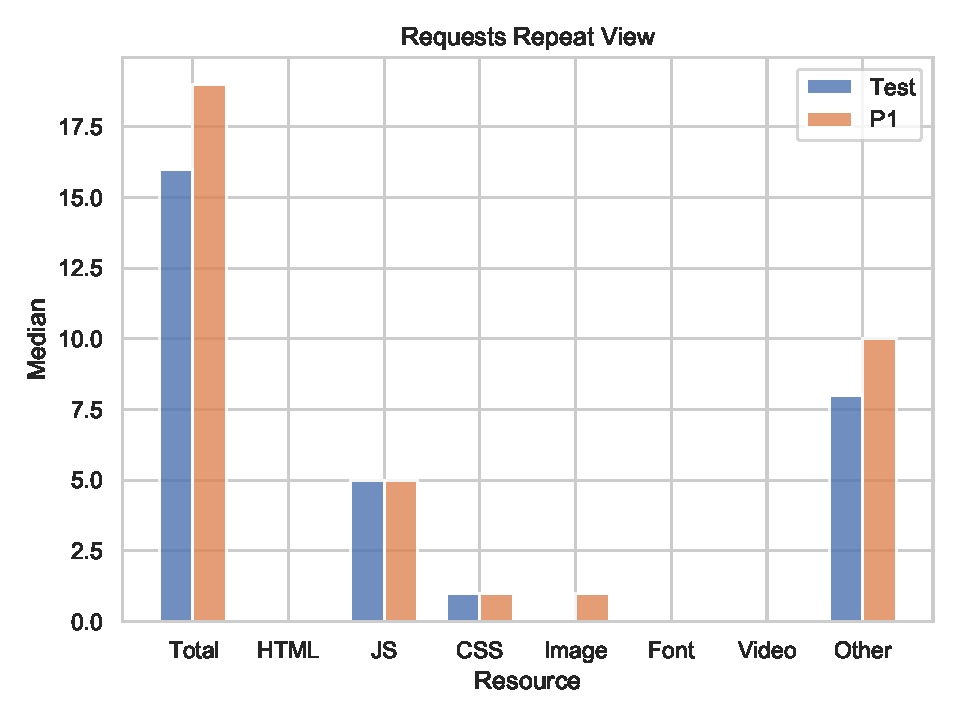
\includegraphics[width=1\linewidth]{plots/original_vs_test/requests_rv.pdf}
		%\caption{Requests}
		\label{fig:sub2}
	\end{subfigure}
	\caption{Page Weight Repeat View, Original vs Test.}
	\label{figure:plt_original_test}
\end{figure}


% --- PLT ---
\begin{figure}
	\centering
	\begin{subfigure}{.5\textwidth}
		\centering
		\includegraphics[width=1\linewidth]{plots/original_vs_test/plt_fv.pdf}
		%\caption{A subfigure}
		\label{fig:sub1}
	\end{subfigure}%
	\begin{subfigure}{.5\textwidth}
		\centering
		\includegraphics[width=1\linewidth]{plots/original_vs_test/plt_rv.pdf}
		%\caption{A subfigure}
		\label{fig:sub2}
	\end{subfigure}
	\caption{Page Load Time, Original vs Test.}
	\label{figure:plt_original_test}
\end{figure}


% --- FCP ---
\begin{figure}
	\centering
	\begin{subfigure}{.5\textwidth}
		\centering
		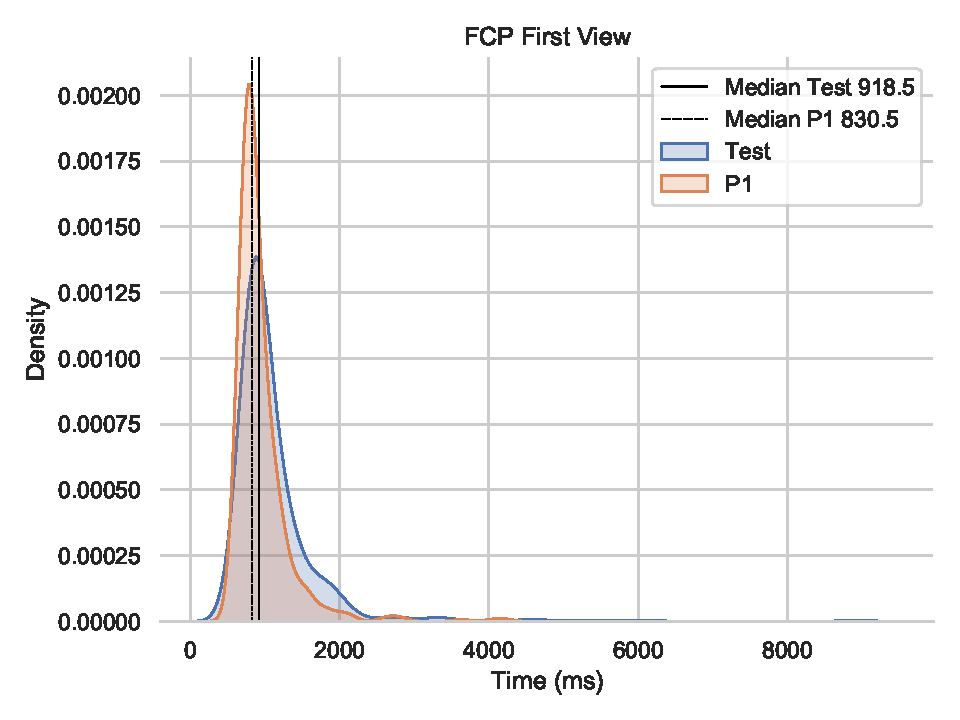
\includegraphics[width=1\linewidth]{plots/original_vs_test/fcp_fv.pdf}
		%\caption{A subfigure}
		\label{fig:sub1}
	\end{subfigure}%
	\begin{subfigure}{.5\textwidth}
		\centering
		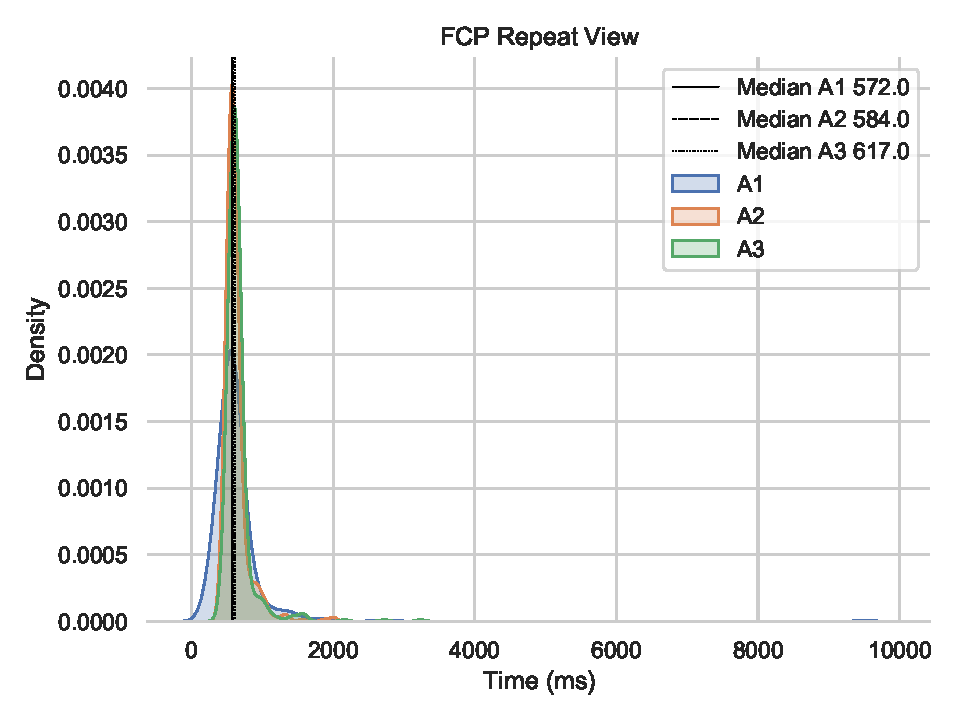
\includegraphics[width=1\linewidth]{plots/original_vs_test/fcp_rv.pdf}
		%\caption{A subfigure}
		\label{fig:sub2}
	\end{subfigure}
	\caption{First Contentful Paint, Original vs Test.}
	\label{figure:fcp_original_test}
\end{figure}

% add LCP / Speed Index ?

\clearpage



\subsection{Test Website without GA vs Variant P1}

% --- Page Weight FV ---
\begin{figure}
	\centering
	\begin{subfigure}{.5\textwidth}
		\centering
		\includegraphics[width=1\linewidth]{plots/test_vs_position/bytes_fv.pdf}
		\caption{Bytes First View}
		\label{fig:sub1}
	\end{subfigure}%
	\begin{subfigure}{.5\textwidth}
		\centering
		\includegraphics[width=1\linewidth]{plots/test_vs_position/requests_fv.pdf}
		\caption{Requests First View}
		\label{fig:sub2}
	\end{subfigure}
	\caption{Page Weight First View, Test vs Variant P1.}
	\label{figure:plt_original_test}
\end{figure}


% --- PLT ---
\begin{figure}
	\centering
	\begin{subfigure}{.5\textwidth}
		\centering
		\includegraphics[width=1\linewidth]{plots/test_vs_position/plt_fv.pdf}
		%\caption{A subfigure}
		\label{fig:sub1}
	\end{subfigure}%
	\begin{subfigure}{.5\textwidth}
		\centering
		\includegraphics[width=1\linewidth]{plots/test_vs_position/plt_rv.pdf}
		%\caption{A subfigure}
		\label{fig:sub2}
	\end{subfigure}
	\caption{Page Load Time, Test vs Variant P1.}
	\label{figure:plt_original_test}
\end{figure}


% --- LCP ---
\begin{figure}
	\centering
	\begin{subfigure}{.5\textwidth}
		\centering
		\includegraphics[width=1\linewidth]{plots/test_vs_position/lcp_fv.pdf}
		%\caption{A subfigure}
		\label{fig:sub1}
	\end{subfigure}%
	\begin{subfigure}{.5\textwidth}
		\centering
		\includegraphics[width=1\linewidth]{plots/test_vs_position/lcp_rv.pdf}
		%\caption{A subfigure}
		\label{fig:sub2}
	\end{subfigure}
	\caption{Largest Contentful Paint, Test vs Variant P1.}
	\label{figure:plt_original_test}
\end{figure}

\clearpage


\subsection{IV Position: Variant P1 vs Variant P2 vs Variant P3}

% --- DCL ---
\begin{figure}
	\centering
	\begin{subfigure}{.5\textwidth}
		\centering
		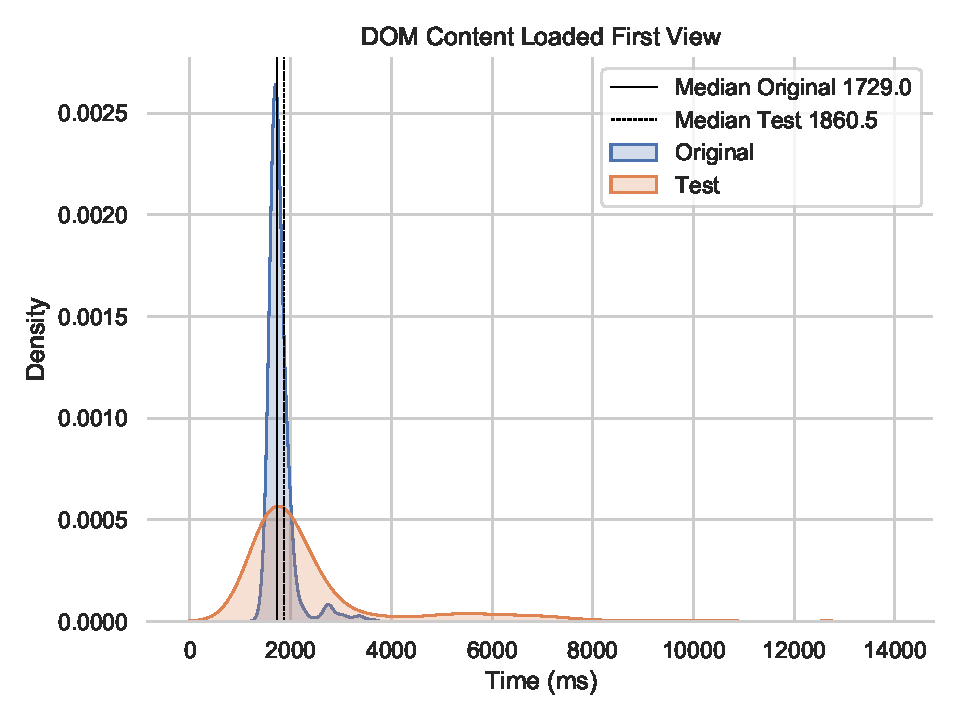
\includegraphics[width=1\linewidth]{plots/IV1_position/dcl_fv.pdf}
		%\caption{A subfigure}
		\label{fig:sub1}
	\end{subfigure}%
	\begin{subfigure}{.5\textwidth}
		\centering
		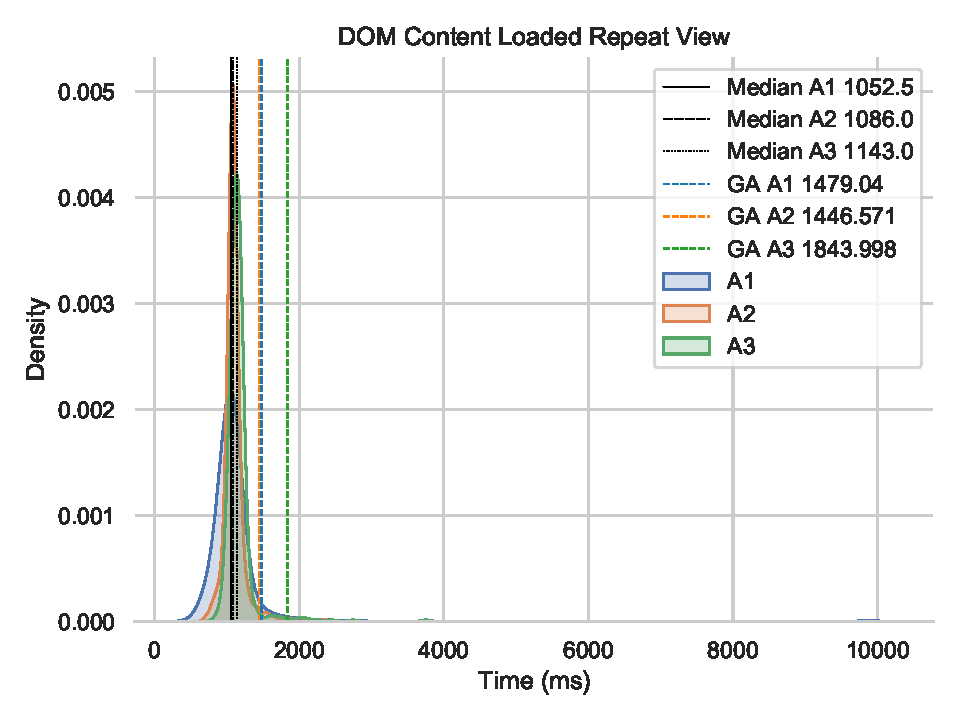
\includegraphics[width=1\linewidth]{plots/IV1_position/dcl_rv.pdf}
		%\caption{A subfigure}
		\label{fig:sub2}
	\end{subfigure}
	\caption{DOM Content Loaded, Variant P1 vs Variant P2 vs Variant P3, with GA.}
	\label{figure:plt_original_test}
\end{figure}


% --- PLT ---
\begin{figure}
	\centering
	\begin{subfigure}{.5\textwidth}
		\centering
		\includegraphics[width=1\linewidth]{plots/IV1_position/plt_fv.pdf}
		%\caption{A subfigure}
		\label{fig:sub1}
	\end{subfigure}%
	\begin{subfigure}{.5\textwidth}
		\centering
		\includegraphics[width=1\linewidth]{plots/IV1_position/plt_rv.pdf}
		%\caption{A subfigure}
		\label{fig:sub2}
	\end{subfigure}
	\caption{Page Load Time, Variant P1 vs Variant P2 vs Variant P3, with GA.}
	\label{figure:plt_original_test}
\end{figure}


% --- SI ---
\begin{figure}
	\centering
	\begin{subfigure}{.5\textwidth}
		\centering
		\includegraphics[width=1\linewidth]{plots/IV1_position/si_fv.pdf}
		%\caption{A subfigure}
		\label{fig:sub1}
	\end{subfigure}%
	\begin{subfigure}{.5\textwidth}
		\centering
		\includegraphics[width=1\linewidth]{plots/IV1_position/si_rv.pdf}
		%\caption{A subfigure}
		\label{fig:sub2}
	\end{subfigure}
	\caption{Speed Index, Variant P1 vs Variant P2 vs Variant P3.}
	\label{figure:plt_original_test}
\end{figure}


% --- LCP ---
\begin{figure}
	\centering
	\begin{subfigure}{.5\textwidth}
		\centering
		\includegraphics[width=1\linewidth]{plots/IV1_position/lcp_fv.pdf}
		%\caption{A subfigure}
		\label{fig:sub1}
	\end{subfigure}%
	\begin{subfigure}{.5\textwidth}
		\centering
		\includegraphics[width=1\linewidth]{plots/IV1_position/lcp_rv.pdf}
		%\caption{A subfigure}
		\label{fig:sub2}
	\end{subfigure}
	\caption{Largest Contentful Paint, Variant P1 vs Variant P2 vs Variant P3.}
	\label{figure:plt_original_test}
\end{figure}


\clearpage



\subsection{IV Attribute: Variant A1 vs Variant A2 vs Variant A3}

%CLS: medians are all the same ??

% --- PLT ---
\begin{figure}
	\centering
	\begin{subfigure}{.5\textwidth}
		\centering
		\includegraphics[width=1\linewidth]{plots/IV2_attribute/plt_fv.pdf}
		%\caption{A subfigure}
		\label{fig:sub1}
	\end{subfigure}%
	\begin{subfigure}{.5\textwidth}
		\centering
		\includegraphics[width=1\linewidth]{plots/IV2_attribute/plt_rv.pdf}
		%\caption{A subfigure}
		\label{fig:sub2}
	\end{subfigure}
	\caption{Page Load Time, Variant A1 vs Variant A2 vs Variant A3, with GA.}
	\label{figure:plt_original_test}
\end{figure}


% --- Fully Loaded ---
\begin{figure}
	\centering
	\begin{subfigure}{.5\textwidth}
		\centering
		\includegraphics[width=1\linewidth]{plots/IV2_attribute/fully_loaded_fv.pdf}
		%\caption{A subfigure}
		\label{fig:sub1}
	\end{subfigure}%
	\begin{subfigure}{.5\textwidth}
		\centering
		\includegraphics[width=1\linewidth]{plots/IV2_attribute/fully_loaded_rv.pdf}
		%\caption{A subfigure}
		\label{fig:sub2}
	\end{subfigure}
	\caption{Fully Loaded, Variant A1 vs Variant A2 vs Variant A3.}
	\label{figure:plt_original_test}
\end{figure}


% --- SI ---
\begin{figure}
	\centering
	\begin{subfigure}{.5\textwidth}
		\centering
		\includegraphics[width=1\linewidth]{plots/IV2_attribute/si_fv.pdf}
		%\caption{A subfigure}
		\label{fig:sub1}
	\end{subfigure}%
	\begin{subfigure}{.5\textwidth}
		\centering
		\includegraphics[width=1\linewidth]{plots/IV2_attribute/si_rv.pdf}
		%\caption{A subfigure}
		\label{fig:sub2}
	\end{subfigure}
	\caption{Speed Index, Variant A1 vs Variant A2 vs Variant A3.}
	\label{figure:plt_original_test}
\end{figure}

% --- LCP ---
\begin{figure}
	\centering
	\begin{subfigure}{.5\textwidth}
		\centering
		\includegraphics[width=1\linewidth]{plots/IV2_attribute/lcp_fv.pdf}
		%\caption{A subfigure}
		\label{fig:sub1}
	\end{subfigure}%
	\begin{subfigure}{.5\textwidth}
		\centering
		\includegraphics[width=1\linewidth]{plots/IV2_attribute/lcp_rv.pdf}
		%\caption{A subfigure}
		\label{fig:sub2}
	\end{subfigure}
	\caption{Largest Contentful Paint, Variant A1 vs Variant A2 vs Variant A3.}
	\label{figure:plt_original_test}
\end{figure}



\clearpage



% -------------------------------------------------------------

\subsection{IV Other Script: Variant OS1 vs Variant OS2}


% --- PLT ---
\begin{figure}
	\centering
	\begin{subfigure}{.5\textwidth}
		\centering
		\includegraphics[width=1\linewidth]{plots/IV3_other_script/plt_fv.pdf}
		%\caption{A subfigure}
		\label{fig:sub1}
	\end{subfigure}%
	\begin{subfigure}{.5\textwidth}
		\centering
		\includegraphics[width=1\linewidth]{plots/IV3_other_script/plt_rv.pdf}
		%\caption{A subfigure}
		\label{fig:sub2}
	\end{subfigure}
	\caption{Page Load Time, Variant OS1 vs Variant OS2, with GA.}
	\label{figure:plt_original_test}
\end{figure}


% --- Fully Loaded ---
\begin{figure}
	\centering
	\begin{subfigure}{.5\textwidth}
		\centering
		\includegraphics[width=1\linewidth]{plots/IV3_other_script/fully_loaded_fv.pdf}
		%\caption{A subfigure}
		\label{fig:sub1}
	\end{subfigure}%
	\begin{subfigure}{.5\textwidth}
		\centering
		\includegraphics[width=1\linewidth]{plots/IV3_other_script/fully_loaded_rv.pdf}
		%\caption{A subfigure}
		\label{fig:sub2}
	\end{subfigure}
	\caption{Fully Loaded, Variant OS1 vs Variant OS2.}
	\label{figure:plt_original_test}
\end{figure}


% --- SI ---
\begin{figure}
	\centering
	\begin{subfigure}{.5\textwidth}
		\centering
		\includegraphics[width=1\linewidth]{plots/IV3_other_script/si_fv.pdf}
		%\caption{A subfigure}
		\label{fig:sub1}
	\end{subfigure}%
	\begin{subfigure}{.5\textwidth}
		\centering
		\includegraphics[width=1\linewidth]{plots/IV3_other_script/si_rv.pdf}
		%\caption{A subfigure}
		\label{fig:sub2}
	\end{subfigure}
	\caption{Speed Index, Variant OS1 vs Variant OS2.}
	\label{figure:plt_original_test}
\end{figure}


% --- TBT ---
\begin{figure}
	\centering
	\begin{subfigure}{.5\textwidth}
		\centering
		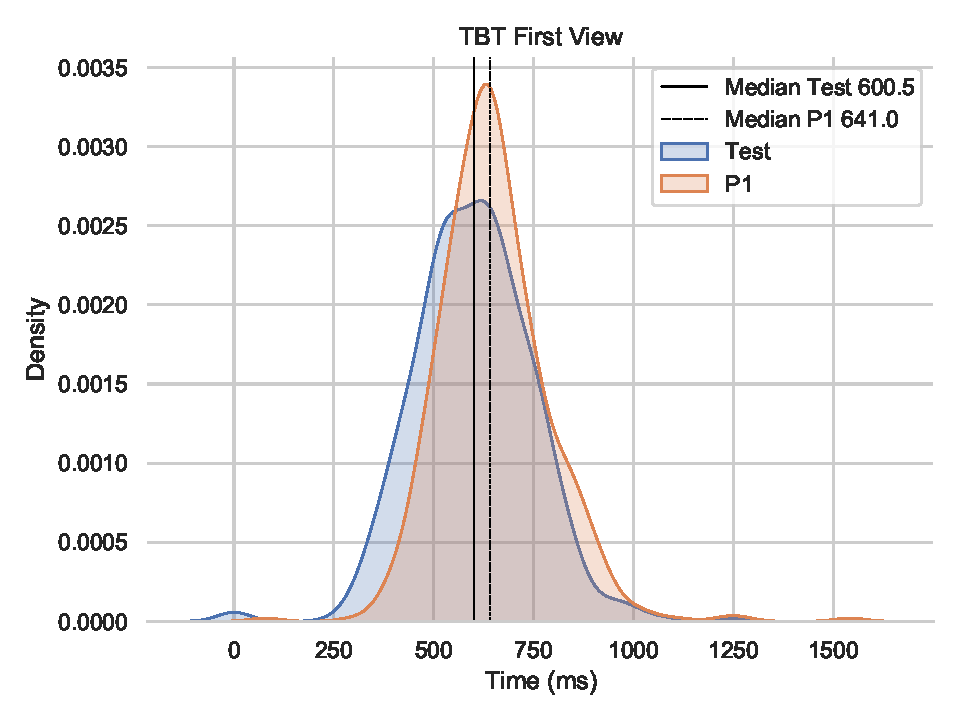
\includegraphics[width=1\linewidth]{plots/IV3_other_script/tbt_fv.pdf}
		%\caption{A subfigure}
		\label{fig:sub1}
	\end{subfigure}%
	\begin{subfigure}{.5\textwidth}
		\centering
		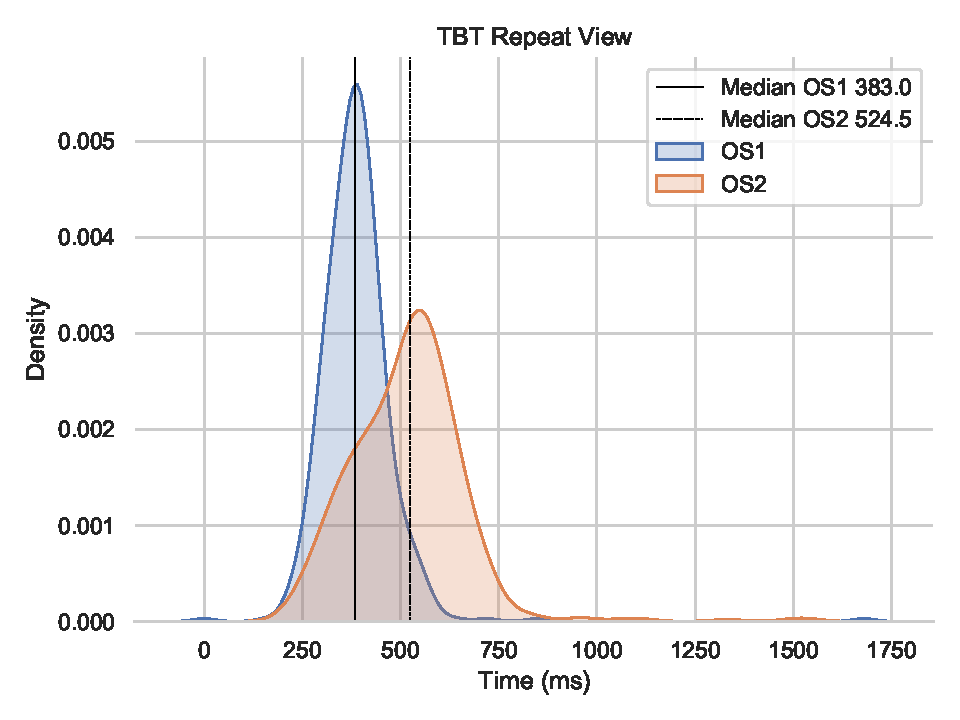
\includegraphics[width=1\linewidth]{plots/IV3_other_script/tbt_rv.pdf}
		%\caption{A subfigure}
		\label{fig:sub2}
	\end{subfigure}
	\caption{Total Blocking Time, Variant OS1 vs Variant OS2.}
	\label{figure:plt_original_test}
\end{figure}

\clearpage


